\section{Interfejs użytkownika}

Interfejs został wykonany w technologii \textbf{Swing}. Główne okna aplikacji to:

\begin{itemize}
    \item \textbf{Ekran logowania} – umożliwia dostęp tylko zalogowanym użytkownikom;
    \item \textbf{Panel sekretariatu} – pozwala na przeglądanie i zarządzanie zajęciami;
    \item \textbf{Formularz dodawania zajęć} – umożliwia wprowadzenie nowych zajęć;
    \item \textbf{Formularz edycji zajęć} – pozwala na modyfikację istniejących rekordów.
\end{itemize}

\section{Walidacja i błędy}

System zawiera zabezpieczenia:

\begin{itemize}
    \item Sprawdzanie dostępności sali w wybranym dniu i godzinie;
    \item Sprawdzanie, czy dana grupa nie ma już zajęć w tym czasie;
    \item Obsługa wyjątków SQL i wyświetlanie komunikatów błędów użytkownikowi.
\end{itemize}

\section{Szczegółowy opis komponentów GUI}

\subsection {Formularz Dodawania Zajęć (DodajZajeciaPanel)}

\begin{itemize}
    \item \textbf{Cel:} Dodawanie nowych rekordów zajęć do bazy danych.
    \item \textbf{Elementy:}
    \begin{itemize}
        \item \texttt{JComboBox} – typ zajęć (np. Wykład, Laboratorium, Projekt);
        \item \texttt{JTextField} – kierunek, przedmiot, prowadzący, sala, godzina, grupa1, grupa2;
        \item \texttt{JComboBox} – dzień tygodnia;
        \item \texttt{JButton} – „Zapisz” — zapisuje dane do bazy danych.
    \end{itemize}
    \item \textbf{Uwagi:} Interfejs zawiera etykiety (\texttt{JLabel}) przypisane do każdego pola. Formularz obsługuje walidację przed zapisem zajęć.
\end{itemize}

\subsection {Formularz Edytowania Zajęć (EdytujZajeciaPanel)}

\begin{itemize}
    \item \textbf{Cel:} Edytowanie istniejących danych zajęć.
    \item \textbf{Elementy:} Te same co w \texttt{DodajZajeciaPanel}, jednak służą do aktualizacji danych:
    \begin{itemize}
        \item Pola są wstępnie wypełnione danymi z wybranego rekordu;
        \item \texttt{JButton} – „Zapisz” — aktualizuje dane w bazie.
    \end{itemize}
    \item \textbf{Uwagi:} Pola są edytowalne i automatycznie uzupełniane na podstawie danych wybranych z tabeli.
\end{itemize}

\subsection {Formularz Logowania (Login)}

\begin{itemize}
    \item \textbf{Cel:} Autoryzacja użytkownika w systemie.
    \item \textbf{Elementy:}
    \begin{itemize}
        \item \texttt{JTextField} – login;
        \item \texttt{JPasswordField} – hasło;
        \item \texttt{JButton} – „Zaloguj” — weryfikuje dane logowania.
    \end{itemize}
    \item \textbf{Uwagi:} Prosty, nowoczesny wygląd z ikoną kłódki; Zabezpieczenie dostępu do aplikacji.
\end{itemize}

\subsection {Panel Sekretariatu (SekretariatPanel)}

\begin{itemize}
    \item \textbf{Cel:} Zarządzanie zajęciami (CRUD).
    \item \textbf{Elementy:}
    \begin{itemize}
        \item \texttt{JTable} – wyświetlanie listy zajęć;
        \item \texttt{JComboBox} – filtrowanie po sali, grupie, typie zajęć;
        \item \texttt{JButton} – „Dodaj”, „Usuń”, „Edytuj”, „Zastosuj filtry”, „Odśwież”;
        \item \texttt{JScrollPane} – przewijana tabela;
        \item \texttt{JLabel} – etykiety opisowe.
    \end{itemize}
    \item \textbf{Uwagi:} Obsługuje filtrowanie i pełną obsługę CRUD; główny ekran zarządzania.
\end{itemize}

\section{Diagram komponentów GUI i zależności}
\vspace{1em}
\noindent\textbf{Diagram komponentów GUI i zależności}

\vspace{0.5em}
\begin{figure}[H]
    \centering
    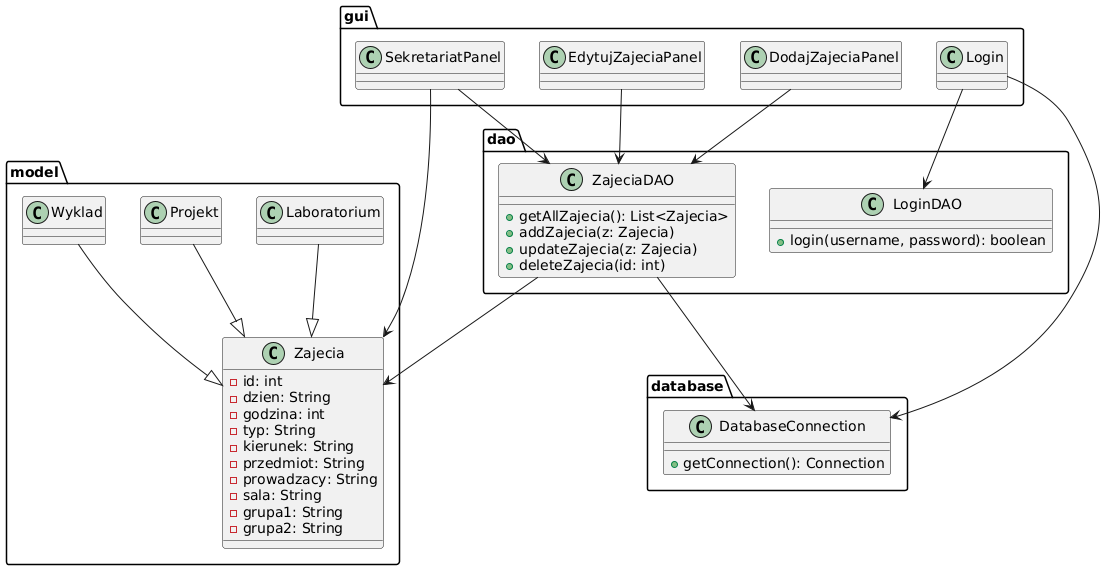
\includegraphics[width=0.95\textwidth]{figures/diagram.png}
    \caption{Zależności pomiędzy komponentami GUI, modelem danych i warstwą DAO}
    \label{fig:diagram-gui}
\end{figure}
